This chapter gives a theoretical foundation and state of the field for the technical domains of relevance for this project: client-side storage, distributed storage, communication, and cryptography. In all fields, standards and technologies for web applications are being rapidly developed and the boundaries for what is possible to achieve in a web application are being continously pushed by browser vendors and standards groups. The goals of Rymd has indeed become technically viable in a web environment as of very recently.

% Client-side storage
The development of client-side data storage in HTML5 is an area that has become more stable and supported across browsers and vendors. Web applications can utilize offline storage like databases (WebSQL and IndexedDB), key-value stores (Web Storage), and even access to the local file system (FileSystem). Under section~\ref{sec:clientstorage}, all of these technologies are presented.

% Distributed storage
Some of the new \emph{cryptocurrencies} can be utilized for distributed storage of data like cryptographic keys. Namecoin and Ethereum are notable examples. In section~\ref{sec:distributedstorage}, they are presented together with Keybase, a service specialized for this purpose that uses a different approach of verifying identities through links at social media accounts.

% Communication
There has been a steady progression in the introduction of communication protocols available for web applications. From client-server HTTP requests (XMLHttpRequest) via client-server full-duplex TCP connections (WebSocket), it has recently become possible with peer-to-peer real-time communication (WebRTC). In section~\ref{sec:communication}, these technologies are presented. Also, issues with NAT traversal in peer-to-peer communication and how they are addressed in WebRTC are explained.

% Crypto
Also of interest, the still unfinalized WebCrypto API~\cite{WebCrypto:Online} has become available in an experimental stage in recent months. In section\ref{sec:techcryptography}, the basics of public-key cryptography and certificates are explained, together with the Web Cryptography API and the Advanced Encryption Standard as part of a symmetric encryption scheme.

% %%%%%%%%%%%%
\section{Client-side storage}
\label{sec:clientstorage}

Client-side storage is how arbitrary data can be persisted on disk, accessible through an API, by a web browser. This is a general term for several separate but related APIs:

\begin{description}
  \item[Web Storage]~\cite{WebStorage:Online} is a simple key-value store in the HTML5 specification.
  \item[WebSQL Database]~\cite{WebSQL:Online} is an embedded SQL relational database.
  \item[FileSystem]~\cite{FileSystem:Online} is an API providing direct file system access.
  \item[Indexed Database]~\cite{IndexedDB:Online}, or \emph{IndexedDB}, is a NoSQL asynchronous data store.
\end{description}

All of these technologies offer ways of storing data on the user's hard drive instead of on a remote server. There are two main reasons for this: to make the application available offline and to improve performance (fewer requests to a server). Older storage techniques include cookies, plugin based storage (Java, Flash, Google Gears) or browser-specific features.

All four APIs tie data to a single \emph{origin}, a practice referred to as \emph{Same Origin Policy}. An origin is defined by the transfer protocol, the domain, and the port number of a website. Thus every data store is associated with an origin, which implicates certain security aspects: an application in \emph{http://domain.com/subdir} may retrieve data from \emph{http://domain.com/subdir/dir} since they have the same origin, but cannot retrieve data from \emph{https://domain.com:3000} due to the different protocol and port number. This is a layer of protection against Cross Site Scripting (XSS) attacks. Note that this is no prevention against XSS holes in the other parts of the application, since a user might be attacked from malicious scripts injected elsewhere in the application.

In order to prevent malicious flooding of users' hard drives, browsers impose limits on storage capacity. If the application exceeds that limit, the browser typically show a dialog in the interface to let the user increase the the limit. This quota is separated for each origin and storage mechanism. For instance, \emph{sub.domain.com} may be allowed to store 5MB of Web Storage and 25MB of IndexedDB data, while \emph{sub2.domain.com} may have other restrictions.

Both of the database-centered technologies, IndexedDB and WebSQL, support \emph{transactions}. This ensures the integrity of the database by preventing of \emph{race conditions}, a phenomenon where two sequences of operations are applied at the same time, leading to unpredictable results and a database state of dubious accuracy. This is done by locking the database for  writing until a sequence of commands are finished.

Most of the storage formats support synchronous and asynchronous modes. Synchronous mode is blocking, meaning that the storage operation will be executed and completed before the next line of code is executed. Asynchronous operations are non-blocking, performed in the background while the rest of the code is executed, and may be completed at a later stage. Generally a \emph{callback function} is provided and called on completion. This is the traditional approach to work with asynchronous operations in JavaScript, where events and callbacks are used heavily. The JavaScript code snippets in listings~\ref{lst:syncCall} and~\ref{lst:asyncCall} show the difference between synchronous and asynchronous calls.

\begin{Code}
\begin{lstlisting}[caption={Synchronous call}, label={lst:syncCall}]
// Fetch a record with id 10 from a database and store in variable
var result = DB.find(10);
\end{lstlisting}

\begin{lstlisting}[caption={Asynchronous call}, label={lst:asyncCall}]
/*
  Request a record with id 10 from a database, continue execute other code,
  and handle result of the database operation in callback when it has finished
*/
var request = DB.find(10);

request.onsuccess = function(evt) {
  var result = evt.result;
};
\end{lstlisting}
\end{Code}

% Mention WebSQL, IndexedDB, etc.

\subsection{Web Storage}
Web Storage is for persisting data in key-value pairs through a single object in web browsers. The API is as simple as attaching values as strings on properties of the global \texttt{localStorage} object as seen in listing~\ref{lst:localStorage}. The \texttt{localStorage} object persists data through browser sessions, while the \texttt{sessionStorage} object will clear all data when the browser tab or window is closed.

\begin{Code}
\begin{lstlisting}[caption={Use of Web Storage}, label={lst:localStorage}]
// Save an item in the local store
localStorage.foo = "bar";
// or
localStorage.setItem("foo", "bar");

// Retrieve item
var val = localStorage.foo;
// or
var val = localStorage.getItem("foo");

// Delete item
localStorage.removeItem("foo");
\end{lstlisting}
\end{Code}

\subsection{WebSQL}
\label{sec:websql}
WebSQL is the only client-side storage technology mentioned that tries to mimic a traditional SQL relational database. It comes with tables, indexing, transactions, keys, and support for schemas. Regular SQL expressions are used to interact with the database, which means the developer can rely on the vast research that has been made in SQL query optimization (see listing~\ref{lst:websql}). WebSQL is high-performing thanks to indexing. Developers who are used to work with traditional databases can start using it in a familiar manner. However, the use of SQL makes the database vulnarable to SQL injection attacks, unless this is taken into account by the developer.

\begin{Code}
\begin{lstlisting}[caption={Use of WebSQL}, label={lst:websql}]
// Create or open database with name, version, description and size of 2MB
var db = openDatabase('testdb', '1.0', 'Test database', 2 * 1024 * 1024);

// Create table and insert data
db.transaction(function(tx) {
  tx.executeSql('CREATE TABLE IF NOT EXISTS NAMES (id unique, first, second)');
  tx.executeSql('INSERT INTO LOGS (id, first, second) VALUES (1, "Johan", "Brook")');
});

// Retrieve all names and print them
db.transaction(function(tx) {
   tx.executeSql('SELECT * FROM NAMES', [], function(tx, results) {
     var len = results.rows.length, item;

     for (var i = 0; i < len; i++){
       item = results.rows.item(i);
       console.log("Name: " + item.first + " " + item.second);
     }
  }, null);
});
\end{lstlisting}
\end{Code}

\subsection{FileSystem}
\label{sec:filesystem}
The FileSystem API allows for read and write access of files and folders on the user's hard drive. Currently, only Google Chrome has a working implementation of the API. FileSystem is suitable for storing larger binary files, and has good performance thanks to its asynchronous structure. There is no support for transactions or indexing. Its API includes methods for manipulating files and folders, as one would expect from a standard file system (see listing~\ref{lst:filesystem}).

\begin{Code}
\begin{lstlisting}[caption={Use of FileSystem}, label={lst:filesystem}]
// Requesting a sandboxed, persistent file system with a size of 2MB and success callback
window.requestFileSystem(window.PERSISTENT, 2 * 1024 * 1024, function(fs) {
  console.log("Opened filesystem: " + fs.name);

  // Create a text file
  fs.root.getFile("test.txt", { create: true, exclusive: true }, function(fileEntry) {
    console.log("Created " + fileEntry.name + " in " + fileEntry.fullPath);
    // => "Created test.txt in /test.txt"
  });

  // Reading a file
  fs.root.getFile("test.txt", {}, function(fileEntry) {

    // Get a File object and read its contents with FileReader.
    fileEntry.file(function(file) {
      var reader = new FileReader();

      reader.onloadend = function() {
        var contents = this.result;

        console.log(contents);
      };

      reader.readAsText(file);
    });
  });

  // Other methods of FileEntry:
  fileEntry.getMetadata(successCallback, opt_errorCallback);
  fileEntry.remove(successCallback, opt_errorCallback);
  fileEntry.moveTo(dirEntry, opt_newName, opt_successCallback, opt_errorCallback);
  fileEntry.copyTo(dirEntry, opt_newName, opt_successCallback, opt_errorCallback);
  fileEntry.getParent(successCallback, opt_errorCallback);
  fileEntry.toURL(opt_mimeType);

  fileEntry.createWriter(successCallback, opt_errorCallback);
});
\end{lstlisting}
\end{Code}

\subsection{IndexedDB}
\label{sec:indexeddb}
IndexedDB is a transactional indexed client-side database capable of storing different types of data structures with an asynchronous API. IndexedDB is actively developed and implemented in the latest versions of Mozilla Firefox, Google Chrome, Microsoft Internet Explorer and Opera. its specification is a Candidate Recommendation by the W3C, as of July 2013~\cite{IndexedDB:Online}.

\subsubsection{Basic structure}
% Cursors, Object Stores, Indexes
Due to IndexedDB's object-oriented nature, a database includes a set of \emph{object stores}, which act similarly to tables in relational database management systems. An object store can hold \emph{objects} of different types including binary data and JavaScript primitives and objects. Each object has a \emph{key} (either specified by the developer from the objects properties, or automatically generated and managed by the database) that is used for indexing and retrieving records. One or several \emph{indexes} can be created on a store from an objects properties for quick querying. A \emph{cursor} is used to iterate on the resulting set of objects from a query on the store.

% Async API
% -----------
% Requests, Callbacks, Events, NoSQL
The asynchronous API has patterns that might be daunting and seem complex to developers not used to NoSQL structures. Unlike WebSQL, IndexedDB does not support SQL and instead exposes ways for querying and manipulating data via \emph{requests} and \emph{transactions} (see section~\ref{subsec:security}). A positive side of the rejection of SQL is the prevention of SQL injection attacks. This comes at the cost of a steeper learning curve for database developers already experienced with more traditional databases. Queries to the database will not yield the resulting data set. Instead requests are returned, which will trigger \emph{events} when the operation is finished. When an event is triggered a callback can be passed to handle the scenario and use the data. See figure~\ref{lst:indexeddb_use} for common use of IndexedDB.

\begin{Code}
\begin{lstlisting}[caption={Use of IndexedDB}, label={lst:indexeddb_use}]
var request = indexedDB.open("testdatabase");

// On database version migrations
request.onupgradeneeded = function(event) {
  var db = event.target.result;

  // Create an objectStore for this database
  var objectStore = db.createObjectStore("store");
};

// When the database is ready to use
request.onsuccess = function(event) {
  var db = request.result;

  // Insert "foo" in the store
  var insertTransaction = db.transaction(["store"], "readwrite").objectStore("store").put("Foo");

  insertTransaction.onsuccess = function(evt) {
    console.log("Inserted 'foo'");
  };

  // Read value with key "key" from the store
  var readTransaction = db.transaction(["store"], "read").objectStore("store").get("key");
  readTransaction.onsuccess = function(evt) {
    console.log("Found " + evt.target.result);
  };
};
\end{lstlisting}
\end{Code}

\subsubsection{Security and reliability}
\label{subsec:security}
IndexedDB is built on a transactional model. This means that all commands run inside a transaction context. Transactions have a certain lifetime and cannot be used after they expire. This transactional model is especially useful for when several instances of a client application are using the same database and issuing commands: Without transactions, concurrency problems and other collisions might occur with data loss as a result. Transactions are able to abort and roll back the database to the state it was in before the transaction was started, should an error occur.

Kimak, Ellman and Laing highlight four important aspects of securing a IndexedDB driven application in their \emph{An Investigation into Possible Attacks on HTML5 IndexedDB and their Prevention}~\cite{IndexedDBSecurity:2012:Online}:

\begin{itemize}
  \item Client-side data encryption
  \item Input validation
  \item SOP (Same-Origin Policy)
  \item Code analysis
\end{itemize}

The database in IndexedDB does not include any kind of bundled encryption or validation, which means that it is the developer's responsibility to sanitize and encrypt sensitive data before insertion into the store. Encryption is vital for the scenario where the contents of the database are compromised, since the attacker would need access to the encryption key in order to read the information in plaintext. Validation is needed in order to prevent malicious content, such as XSS, from being inserted as the data fields in the store (without the user's knowledge). Properly crafted code could otherwise pose a security risk since vulnerable applications could execute it at a later stage.

Code analysis is divided into \emph{static} and \emph{dynamic} analysis. Static analysis is the analysis of the to-be inserted data in order to detect malicious material. Dynamic analysis is the analysis of executed programs, and can be done by checking the call from the web application to the database. On success, the database operation s allowed to fully execute~\cite{IndexedDBSecurity:2012:Online}.

\section{Distributed storage}
\label{sec:distributedstorage}
With the inherent problems of trust in CAs in a PKI, several approaches to publicly available distribution of cryptographic keys have emerged in recent years. Some use a blockchain-based approach derived from Bitcoin. This implies distributing a cryptographically based ledger over an entire network and taking it beyond that of a monetary currency to systems that can be used for a wider range of applications. There are also other ideas on how to solve the trust issue.

\subsection{Namecoin}
A phenomenon that has been on the rise during recent years is that of cryptocurrencies such as Bitcoin~\cite{nakamoto:2009}. A cryptocurrency is a virtual currency that builds on cryptographical principles to ensure integrity and consistency. Each participant in the Bitcoin network keeps a ledger of all transactions throughout the history of the network. This ledger is called the \emph{blockchain}, because it is a chain of \emph{blocks}. Each block constitutes of the hash of the previously generated block, a number of other recent transactions and a salt. In order for a transaction to be deemed valid, it needs to be included in one of these blocks. This inclusion is done by volunteering nodes that perform a brute-force search for a salt that generates a block hash of a specific form. When such a salt has been found, the block is included in the blockchain. This search for salts is called \emph{mining} and constitutes the work done by \emph{miners} to keep the network running. As an incentive, each verified block also includes a reward to the miner that finds the salt. In effect, all transactions ever made are publicly available and tracked so that anyone can confirm their validity. This prevents forgery and double-spending of bitcoins.

Namecoin~\cite{Namecoin:Online}, another cryptocurrency, is essentially a fork of Bitcoin with new transaction types that allows its blockchain to be utilized as a distributed key-value store. Although similar in nature to Bitcoin, its main purpose is to be used as a decentralized domain name system (DNS), rather than as a monetary currency.

With a decentralized DNS such as Namecoin, top level domains (such as \emph{.com} or \emph{.se}) can exist without being controlled by any central authority~\cite{Coindesk:2013:Online}. Also, the DNS lookup tables where domain names and their IP addresses are stored are shared in a peer-to-peer manner. The only necessary condition for these domains to be accessible is that there are participants willing to run the DNS server software. Although mainly intended to be used as a DNS, it contains several namespaces where arbitrary strings such as public cryptographic keys can be stored.

\subsection{Ethereum}
Bitcoin and its derivatives have a built-in scripting language that runs on top of the blockchain. It has limited functionality and is mainly used to set up contracts and multi-party-signed transactions that enables escrow-like functionality. Ethereum~\cite{Ethereum:Online} is a novel crypto-currency built from scratch that extends this idea by building on \emph{smart contracts} using a Turing complete domain specific language. This makes it a platform for buildig arbitrary distributed system. Users running code pay a small fee of the internal currency \emph{ether} for each computational step. Ethereum could therefore work not only as a DHT, but also execute parts of system logic. Development of Ethereum was annunced at the end of 2013 and has a planned first release in late 2014.

\subsection{Keybase}
Keybase~\cite{Keybase:Online} is another recent initiative that intends to solve the distribution of public keys. It is essentially an HTTP-interface that maps keys to identities. While keys themselves are stored centrally at Keybase's servers, it utilizes social media for proofs. The idea is that a Keybase user will put proofs of their Keybase identity on public social media services like Twitter or Github. The Keybase client will refer to these to make sure that the given key corresponds to the user of these social media accounts. It ties identities to keys as long as a user's Keybase and social media accounts are not all compromised.


\section{Communication}
\label{sec:communication}
In the beginning of the World Wide Web's history, web browsers performed full page loads in order to render web pages. Further down the road, techniques such as AJAX (Asynchronous JavaScript and XML) enabled data to be fetched asynchronously from servers through the XMLHttpRequest API, thereby unlocking the creation of dynamic web applications. Since then, we have witnessed the introduction of the WebSocket protocol which enables persistent two-way communication between client and server. These techniques are centered around communication between a client and a server, but with the recent initiative of WebRTC (Web Real-Time Communication) which enables peer-to-peer communication there are some new possibilities in the field. In order to understand how these techniques work, some inherent problems with the infrastructure of the internet will be discussed in the NAT Traversal section.

\subsection{XMLHttpRequest}
XMLHttpRequest (XHR) is a browser API which enables data to be fetched asynchronously from servers. This means that a web page can retrieve new updates from the server without a full page reload. The browser is responsible for the construction of HTTP requests according to parameters passed to the API. In the use case where real-time updates from the server are desired, a common technique is to poll the server at regular intervals as the possibilities for streaming are limited. Although the name of the API suggests that data transfers are limited to XML, this is not the case and the name is nothing more than a remnant of the past~\cite{XHR:Online}. Today it is much more common to transport data in the form of JavaScript-serialized objects, also known as \emph{JSON} (JavaScript Object Notation).

\subsection{WebSocket}
WebSocket (RFC 6455)~\cite{RFC6455:Online} is a protocol which was standardized in 2011. The protocol allows two way communication between a server and a client through persistent connections. The protocol runs on top of the TCP protocol and is independent from the HTTP protocol. The implications of this is that the server does not need to open a new TCP connection for every incoming message as in XHR, and the high overhead from HTTP is eliminated which eases server workload.

\subsection{NAT Traversal}
\label{subsec:nattraversal}
% rewrite so its not centered around webrtc
Network Address Translation (NAT)~\cite{RFC1631:Online} was first introduced as as a short-term solution to the problem of IP address depletion in IPv4. The idea was that by utilizing NATs, several hosts in a private network could share a single public IP address.

A NAT is responsible for maintaining a table of entries that map an internal IP address and port to a public IP address and port and dropping these entries when they are no longer of relevant. When a host behind a NAT wants to communicate with an external host, the NAT creates an entry in the table which can then be used to route the response back to the internal host(See figure~\ref{fig:NAT})~\cite{RFC5245:Online}.

\begin{figure}[htp]
\centering
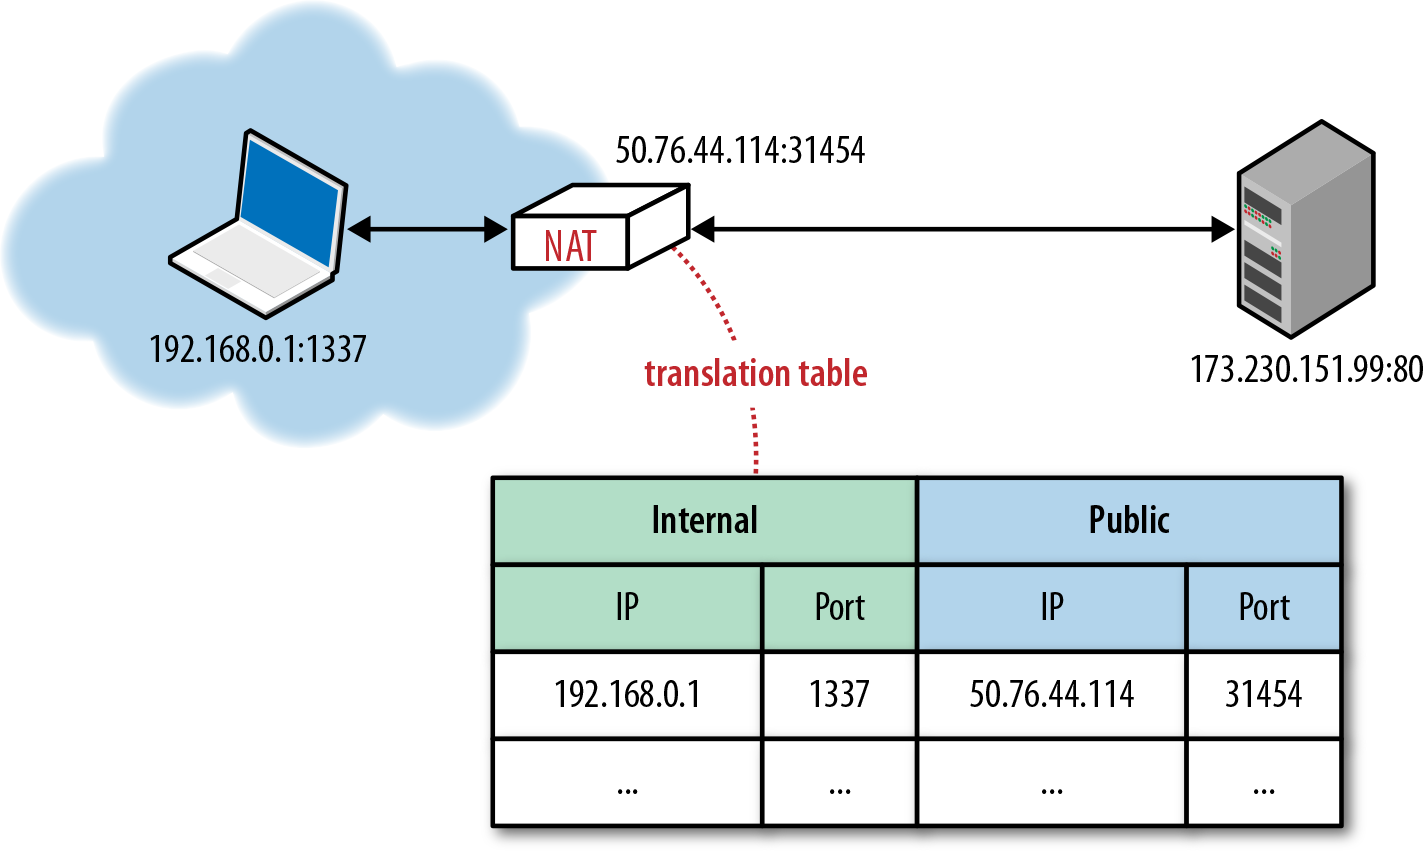
\includegraphics[width=\textwidth,height=0.2\paperheight,keepaspectratio
]{figures/nat}
\caption{A NAT maintains a table mapping internal IP and port, to a public IP and port.~\cite{NATIllustration:Online}.}
\label{fig:NAT}
\end{figure}

The presence of NATs can pose a problem to applications leveraging the UDP protocol for transportation of data and network communication in general. The different techniques that can be used to resolve problems caused by NATs are often referred to as \emph{NAT Traversal} techniques.

The underlying issue with the UDP protocol is the absense of state, as opposed to the TCP protocol. The statelessness of the UDP protocol makes it difficult for a NAT to determine when a table entry is no longer relevant and should be dropped, which leads to the fact that UDP routing entries are expired based on time. If an entry is predeterminedly expired, it will cause inbound packets to be dropped since they cannot reach the source. In the case of TCP, which constitutes a well defined state, it is inherently simple to determine when an entry should be dropped.

A technique commonly used to solve the problem with UDP entries expiring and being dropped is to utilize keepalives at regular intervals. This is is commonly referred to as \emph{UDP hole punching}~\cite{UDPHolePunching:Online}.

Another problem is that internal hosts know their internal IP address but not their public one. If a host runs an application that communicates the IP address as a part of the payload to hosts oustide of the private network, there would obviously be a missmatch if the internal address is chosen. Therefore it is common to utilize a protocol called STUN (Session Traversal Utilities for NAT)~\cite{RFC5389:Online}. STUN enables hosts to obtain their public IP addresses with the help of an external STUN server (See figure~\ref{fig:WebRTC - STUN}).

\begin{figure}[htp]
\centering
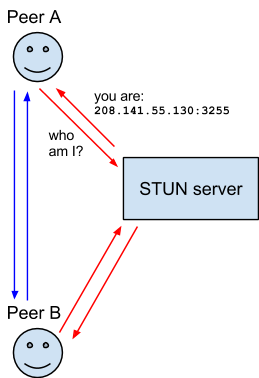
\includegraphics[width=\textwidth,height=0.2\paperheight,keepaspectratio
]{figures/webrtc-stun}
\caption{STUN servers let peers in a private network behind firewalls discover their public IP-addresses~\cite{WebRTCArchitecture:2014:Online}.}
\label{fig:WebRTC - STUN}
\end{figure}

These techniques are not always adequate because of the fact that STUN does not work with all types of NATs. In some cases, UDP traffic might be blocked by a firewall. This is where the TURN (Traversal Using Relays around NAT) protocol~\cite{RFC5766:Online} can be leveraged.  TURN establish a TCP connection with a relay server when UDP has failed. The relay server is used to tunnel data to the other host, which means that there is no longer a direct peer-to-peer connection (See figure~\ref{fig:WebRTC - TURN}).

\begin{figure}[htp]
\centering
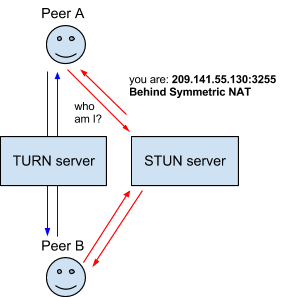
\includegraphics[width=\textwidth,height=0.2\paperheight,keepaspectratio
]{figures/webrtc-turn}
\caption{If a peer-to-peer connection cannot be established, a relay through a TURN server could be used. All peers send their packets through the relay which makes it more costly. But at least the connection works~\cite{WebRTCArchitecture:2014:Online}.}
\label{fig:WebRTC - TURN}
\end{figure}

\subsection{WebRTC}

Up until recently, browsers have lacked support for direct peer-to-peer communication. Then in 2011 Google released a project called WebRTC, with the purpose of enabling real-time voice and video in the browser~\cite{WebRTCMemo:Online}. Since then, WebRTC has evolved to enable more general real-time data communication between browsers~\cite{WebRTC:Online}. It has become usable for arbitrary data streams in major browsers in 2014~\cite{WebRTCChrome:Online}~\cite{WebRTCFirefox:Online}.

Since the announcement of WebRTC, the organizations W3C and IETF have worked together on standardizing protocols and drafting APIs. The major browser vendors Google, Mozilla and Opera support the project~\cite{WebRTCAndMicrosoft:2012:Online}. While Microsoft supports the concept of WebRTC and contributes to the W3C WebRTC working group, it does not support Google's (or nowadays, W3C's and IETF's) version of it~\cite{WebRTCAndMicrosoft:2012:Online}. Microsoft doesn't want to support the new technology until it has become a standard and does not fully agree on some constraints placed on it~\cite{WebRTCAndMicrosoft:2012:Online}. Microsoft states that one of their issues with the current WebRTC version is that it has predetermined paths for choosing codecs and ways of sending media over the network – sort of a black box. This hinders application developers who want to optimize to suit their own needs. Microsoft's answer to this is their own CU-RTC-WEB (Customizable, Ubiquitous Real Time Communication over the Web) which attempts to address these issues.

WebRTC's functionality is abstracted into three different APIs: \emph{MediaStream}, \emph{RTCPeerConnection} and \emph{RTCDataChannel}~\cite{WebRTCBasics:2012:Online}. MediaStream, or \emph{getUserMedia}, handles synchronized media streams, i.e. synchronized video and sound from a computer's camera and microphone. RTCPeerConnection manages reliable and efficient communication of the data streams, it utilizes techniques such as \emph{jitter buffering} and \emph{echo cancellation} to ensure a high standard even in unstable networks. For the intent of file sharing, the RTCDataChannel API is the most relevant.

% Introduce that WebRTC builds on top of UDP
At the transport layer WebRTC makes use of UDP which can be motivated by the fact that timeliness is vital for real-time communication~\cite{HighPerfBrowserNetworking:Online}. The UDP protocol alone is not enough to construct efficient peer-to-peer applications. For this very reason, WebRTC leverages a number of additional protocols built on top of UDP (See figure~\ref{fig:WebRTCProtocols}).

WebRTC's usage of UDP makes peer-to-peer communication inclined to suffer from connectivity problems in the presence of NATs (see section~\ref{subsubsec:rtcpeerconnection}). This problem has been taken into account and is relieved by utilizing the ICE protocol (see section~\ref{subsubsec:rtcpeerconnection}).

For the sake of security, data is encrypted according to the DTLS (Datagram Transport Layer Security) protocol. The DTLS protocol is based on the TLS (Transport Layer Security) protocol, the main difference being that DTLS is constructed for datagrams while TLS is used for reliable transport protocols such as TCP.
% udp does not guarantee that much, introduce some other protcols that helps

% insert protocol stack
\begin{figure}[htp]
\centering
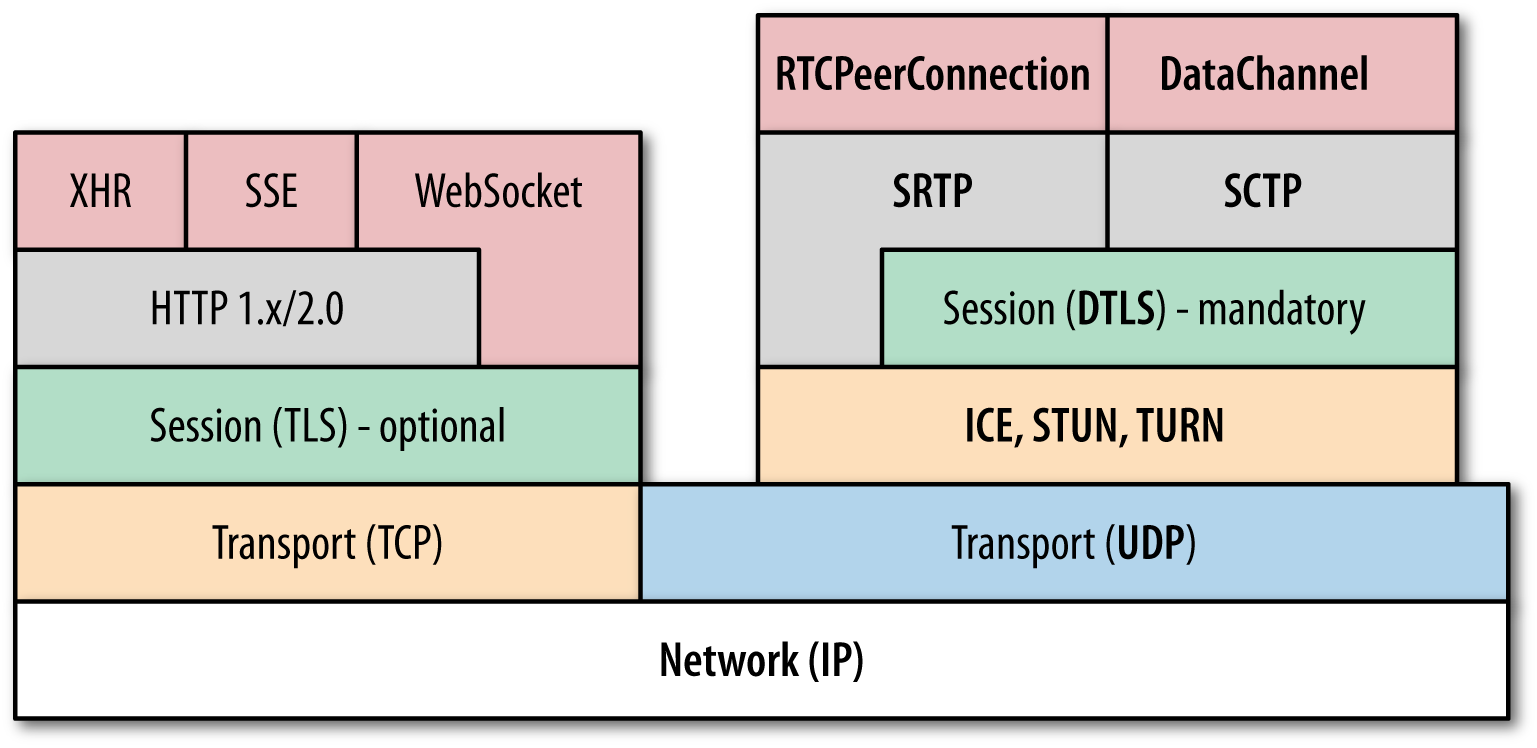
\includegraphics[width=\textwidth,height=0.25\paperheight,keepaspectratio
]{figures/webrtc_protocol_stack}
\caption{WebRTC's underlying protocols~\cite{WebRTCProtocolStack:Online}}
\label{fig:WebRTCProtocols}
\end{figure}

% Data transfers are encrypted with the DTLS protcol

\subsubsection{RTCPeerConnection}
\label{subsubsec:rtcpeerconnection}
The RTCPeerConnection API handles the creation of peer-to-peer connections and takes care of connectivity problems caused by NATs (see section~\ref{subsec:nattraversal}) by utilizing the Interactive Connection Establishment (ICE) protocol~\cite{RFC5245:Online}. The ICE protocol handles \emph{NAT Traversal} and is used for establishing peer-to-peer connections. It makes use of STUN and falls back to TURN when no other alternatives exists (See figure~\ref{fig:ICE}).

\begin{figure}[htp]
\centering
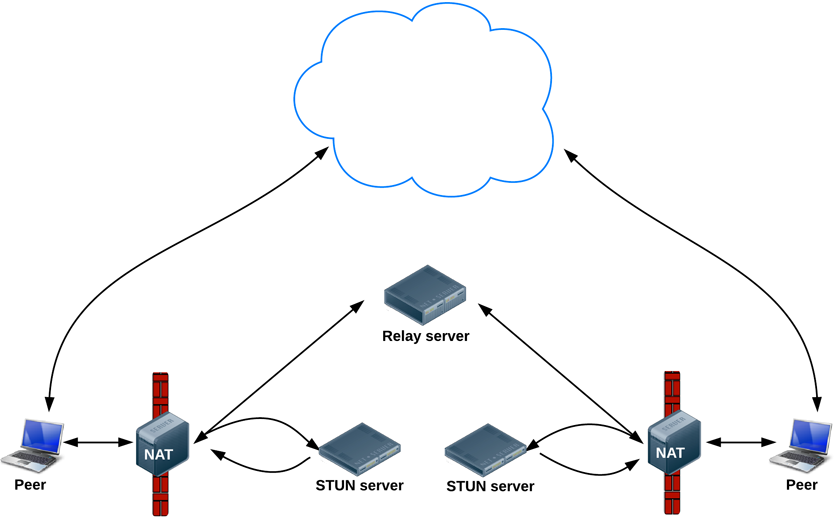
\includegraphics[width=\textwidth,height=0.25\paperheight,keepaspectratio
]{figures/ICE}
\caption{{The different ways for ICE to find network interfaces and ports, titled \emph{Finding connection candidates}~\cite{WebRTCBasics:2012:Online}, available under a Creative Commons Attribution 3.0 Unported License\protect\footnotemark}}
\label{fig:ICE}
\end{figure}

\footnotetext{http://creativecommons.org/licenses/by/3.0/legalcode} %Footnote text to ICE figure caption

Before a connection can be initiated between peers, one of two parts must extend an offer which contains data describing the connection to the other part - this is often referred to as the signaling phase. The signaling phase depends on two things:

\begin{itemize}
  \item The existence of a signaling channel - where a connection should be negotiated
  \item The choice of signaling protocol - which protocol that should be used for the negotiation
\end{itemize}

Regarding the choice of signaling channel, a dedicated signaling server is often used. That is, a server which relays connection offers from one peer to another. Although this is the most common choice of signaling channel, examples of a more serverless approach can be found~\cite{webrtcsignalserver}. For the choice of signaling protocol the standard does not provide any recommendations - this is for developers to decide.

\subsubsection{RTCDataChannel}
The RTCDataChannel API allows for arbitrary data to be sent peer-to-peer by leveraging the RTCPeerConnection API. As UDP itself, which WebRTC runs on top of, is not suitable for reliable data transportation the RTCDataChannel API utilize the SCTP (Stream Control Transport Protocol) protocol. SCTP can be configured in terms of reliability and message order, and it provides some additional services such as congestion and flow control~\cite{HighPerfBrowserNetworking:Online}.

\section{Cryptography}
\label{sec:techcryptography}
Encryption is the process of running data through an algorithm with the goal of making the information unreadable for unauthorized parties. The output of an algorithm depends on the input data and the \emph{encryption key} used. There are two types of key schemes: symmetric-key schemes and asymmetric-key schemes (also known as public-private). In symmetric cryptography  schemes such as AES, the same key is used for both encryption and decryption. Because of this, both sender and recipient must possess the same key, and the key must therefore somehow be communicated through a secure channel. Asymmetric key-schemes like RSA, on the other hand, work with pairs of keys where the encryption of one corresponds to the decryption of the other. One of these keys is called \emph{private} and should only be known to the person generating the key-pair, and the other is called \emph{public} and can be shared freely. In this way, there is no problem with how to transmit keys. Generally, encryption and decryption in asymmetric schemes are much more computationally demanding than that of symmetric schemes, so a common approach is to use symmetric encryption for data and asymmetric keys for the communication of the symmetric key.

Until recently, the practice of performing cryptographic operations in a web browser environment has been considered bad practice by security professionals~\cite{Matasano:Online}. One reason for this is that it has been impossible to verify the integrity of client-side source code between executions - something that has now changed with the advent of signed browser extensions. Another issue is the internal openness of JavaScript - any cryptographic implementation would unavoidably expose all their primitives\footnote{The basic functions in a cryptographic scheme such as hashing, encryption, decryption, signing, verification and generation of keys}, as well as raw private and secret key data. With the advent of the new Web Cryptography API, or \emph{WebCrypto}, these issues are being addressed~\cite{WebCrypto:Online}.

\subsection{Web Cryptography API}
WebCrypto is an open standard for implementation of cryptographic primitives accessible through web client code~\cite{WebCrypto:Online}. Basically, all primitives and raw material (the underlying keys and algorithms) would be blackboxed for the client application and executed natively in the web browser. However, the API is still in an early stage and at the time of this writing only Chromium~\cite{ImplementedChromium:Online} and Microsoft Internet Explorer~\cite{WCAImplementationMicrosoft:Online}, out of the major browsers have implemented more than a basic pseudo-random number generator~\cite{WCAImplementationMozilla:Online}. The exact implementation of the different features may come to change drastically over time.

\subsection{Certificates}
% TODO: Explain usage of X.509 and why it's relevant
Certificates are used to confirm the validity of users' keys~\cite{EETimesCrypto:Online}. Instead of requesting keys directly, which could have potentially been compromised by malicious third parties, certificates are retrieved from trusted CAs. In essence, a certificate contains a user's public key along with user data and information about the certificate. The CA signs the certificate and a hash is embedded as proof that the certificate has not been unlawfully modified.

These certificates are structured according to a certain format. One commonly used format for certificates is the X.509 standard~\cite{IETFX509:Online}. In the X.509 system, a CA issues a certificate binding a public key to a name such as an e-mail address or a DNS entry.

\subsection{Advanced Encryption Standard}

% TODO: Explain relevance of algorithms in general as well as usage of AES and why it's relevant
The Advanced Encryption Standard~\cite{AES:2001}, \emph{AES}, is one of the most widespread symmetric encryption schemes in use today. It is a specification established by the U.S. National Institute of Standards and Technogy in 2001 and based on the Rijndael cipher~\cite{Rijndael:Online}, which in turn is based on the idea of substitution-permutation~\cite{AESISFAST:Online}. The algorithm distorts the inputed value by means of replacement and uses a structure with a fixed block size. AES was intended as a replacement for DES~\cite{DES:1977}~\cite{Cisco:2001}. Encryption is performed in rounds with the number of rounds depending on the length of the key.

For reasons of performance and security, symmetric algorithms such as AES encrypt data in blocks of fixed size. There are different ways to make these blocks relate to each other, depending on the type of data and application. One of the more common modes is Cipher Block Chaining, or CBC, where the encryption function for each subsequent block is fed the encrypted version of the previous block. This is done to make blocks with the same input plaintext indistinguishable~\cite{SearchSecurityCipherBlockChaining:Online}.
% Diffusion and confusions together will complicate statistics attacks and hides local patterns in the language.
